%; whizzy chapter
% -initex iniptex -latex platex -format platex -bibtex jbibtex -fmt fmt
% 以上 whizzytex を使用する場合の設定.

%     Kansai Debian Meeting resources
%     Copyright (C) 2007 Takaya Yamashita
%     Thank you for Tokyo Debian Meeting resources

%     This program is free software; you can redistribute it and/or modify
%     it under the terms of the GNU General Public License as published by
%     the Free Software Foundation; either version 2 of the License, or
%     (at your option) any later version.

%     This program is distributed in the hope that it will be useful,
%     but WITHOUT ANY WARRANTY; without even the implied warranty of
%     MERCHANTABILITY or FITNESS FOR A PARTICULAR PURPOSE.  See the
%     GNU General Public License for more details.

%     You should have received a copy of the GNU General Public License
%     along with this program; if not, write to the Free Software
%     Foundation, Inc., 51 Franklin St, Fifth Floor, Boston, MA  02110-1301 USA

%  preview (shell-command (concat "evince " (replace-regexp-in-string "tex$" "pdf"(buffer-file-name)) "&"))
% 画像ファイルを処理するためには ebb を利用して boundingbox を作成.
%(shell-command "cd image200708; ebb *.png")

%%ここからヘッダ開始.

\documentclass[mingoth,a4paper]{jsarticle}
\usepackage{kansaimonthlyreport}
\usepackage[dvips]{xy}
\usepackage{ascmac}

% 今回限りのコマンド
\definecolor{debianred}{rgb}{.780,.000,.211} % 199,0,54
\definecolor{debianblue}{rgb}{0,.208,.780} % 0,53,199
\definecolor{debianlightbackgroundblue}{rgb}{.941,.941,.957} % 240,240,244
\definecolor{debianbackgroundblue}{rgb}{.776,.784,.878} % 198,200,224
\definecolor{noir}{RGB}{3,3,36}
\definecolor{bleu}{RGB}{10,10,120}
\definecolor{bleuclair}{RGB}{17,17,150}
\definecolor{rouge}{RGB}{200,0,0}
\definecolor{jaune}{RGB}{255,255,0}
\definecolor{vert}{RGB}{0,255,0}
\definecolor{rougebg}{RGB}{160,0,0}
\definecolor{darkred}{rgb}{.7,0,0}
\newcommand{\textttc}[1]{\texttt{\color{rouge}#1}}
\newcommand{\textalert}[1]{{\color{darkred}{#1}}}
\usepackage{listings}
\lstset{basicstyle=\ttfamily}
\newcommand{\seprule}{\vspace*{-0.5em}\centerline{\rule{\linewidth}{0.3pt}}\vspace*{-0.5em}}
% 今回限りのコマンド

% 日付を定義する, 毎月変わります.
\newcommand{\debmtgyear}{2011}
\newcommand{\debmtgmonth}{08}
\newcommand{\debmtgdate}{28}
\newcommand{\debmtgnumber}{50}

\begin{document}

\begin{titlepage}

% 毎月変更する部分, 本文の末尾も修正することをわすれずに

 第\debmtgnumber{}回 関西 Debian 勉強会資料

\vspace{2cm}

\begin{center}
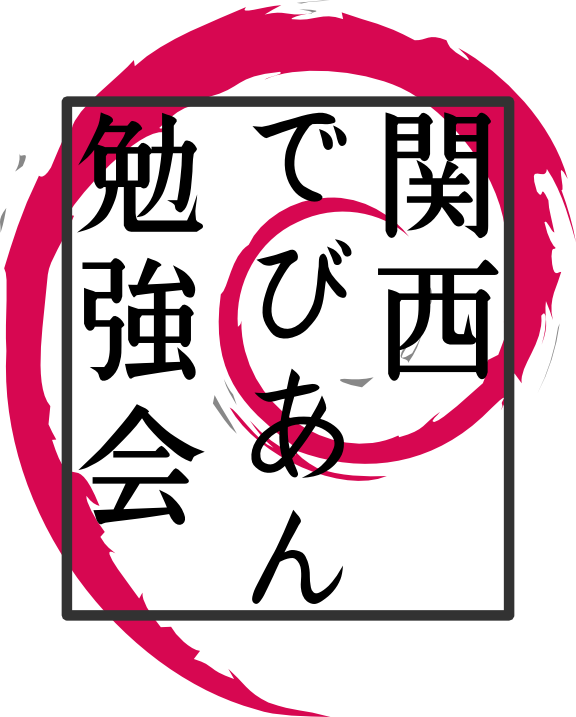
\includegraphics{image200802/kansaidebianlogo.png}
\end{center}

\begin{flushright}
\hfill{}関西 Debian 勉強会担当者 佐々木・倉敷・のがた \\
\hfill{}\debmtgyear{}年\debmtgmonth{}月\debmtgdate{}日
\end{flushright}

\thispagestyle{empty}
\end{titlepage}

\dancersection{Introduction}{Debian JP}

\subsection*{}%ロゴ用のスペース稼ぎ

関西 Debian 勉強会は Debian GNU/Linux のさまざまなトピック (新しいパッケー
ジ, Debian 特有の機能の仕組, Debian 界隈で起こった出来事, などなど) に
ついて話し合う会です.

目的として次の三つを考えています.
\begin{itemize}
      \item ML や掲示板ではなく, 直接顔を合わせる事での情報交換の促進
      \item 定期的に集まれる場所
      \item 資料の作成
\end{itemize}

それでは, 楽しい一時をお楽しみ下さい.

\clearpage

\begin{minipage}[b]{0.2\hsize}
 {\rotatebox{90}{\fontsize{80}{80}
{\gt 関西 Debian 勉強会}}}
\end{minipage}
\begin{minipage}[b]{0.8\hsize}
\hrule
\vspace{2mm}
\hrule
\setcounter{tocdepth}{1}
\tableofcontents
\vspace{2mm}
\hrule
\end{minipage}


\dancersection{最近の Debian 関係のイベント報告}{Debian JP}

\subsection{OSC 2011 Kyoto}

2011年7月16日(土)に京都リサーチパーク(KRP)でオープンソースカンファレンス2011京都が開
催されました。

\subsection{Debconf11}

年に一度の Debian 開発者会議 Debconf が、2011年7月24日〜30日に、ボスニアの Banja Luka で開催されました。
日本からは、東京の勉強会から 3 名ほど参加がありました。勉強会資料で参加レポートを読むことができると思います。

残念ながら関西からの参加者はいませんでしたが、高品質なビデオストリーミングなどもありますので、今からでも見てみると
面白いのではないでしょうか。


\clearpage
%-------------------------------------------------------------------------------
\dancersection{事前課題}{Debian JP}

今回は以下の事前課題を設定しました。


Debian GNU/Linux unstable (sid) が使える環境を用意しておいて下さい。 普段お使いの環境が sid の場合には特に事前課題はありません。普段使いの環境が sid 以外の場合には、以下の方法が考えられます。

\begin{enumerate}

\item VirtualBox などの仮想マシン上に sid を install する
\item (c)debootstrap + schroot で sid 環境へ切り替えられるようにしておく
\item squeeze/wheezy を sid に upgrade する
\end{enumerate}

参加者の皆さんによる回答は以下の通りです。

\begin{prework}{ のがたじゅん }

普段の環境がsidなので、とくになにもしてません。
\end{prework}

\begin{prework}{ 佐々木洋平 }

今更(08/28 08:42) 申し込んでいないことに気がつく愚か者です。

普段から sid 使っています。 schroot もバリバリ。
\begin{commandline}
 $ ls -l /var/chroot
 drwxr-xr-x 22 root root 4096 2011-08-01 08:10 TeXLive-amd64/
 drwxr-xr-x 20 root root 4096 2011-07-14 11:07 lenny-i386/
 drwxr-xr-x 20 root root 4096 2011-07-14 11:07 lenny-amd64/
 drwxr-xr-x 20 root root 4096 2011-05-12 10:07 squeeze-i386/
 drwxr-xr-x 20 root root 4096 2011-05-12 10:07 squeeze-amd64/
 drwxr-xr-x 20 root root 4096 2011-08-14 18:07 sid-i386/
\end{commandline}
%$
\end{prework}

\begin{prework}{ 榎真治 }
(無回答)
\end{prework}

\begin{prework}{ gdevmjc }
久保です.お世話になります。

2. debootstrap + schroot で sid 環境を作ります。

debootstrap は完了。続いて schroot 勉強中。
\end{prework}

\begin{prework}{ 水野源 }

さて、Ubuntu 10.10上にどうやってsid環境作るかね…

\end{prework}

\begin{prework}{ murase\_syuka }

(無回答)

\end{prework}

\begin{prework}{ かわだてつたろう }

ラップトップでは sid 環境を使っています。
たまーに何かあるようですが、普通に使えています。
\end{prework}

\begin{prework}{ ojima.h }

(無回答)

\end{prework}

\begin{prework}{ 甲斐正三 }

持参するPCは事情によりSidにできないので、
今回はハンズオン無しでお話を伺うことになると思いますがよろしくお願いします。
(自宅のPCはホスト"amd64-stable"にkvm-qemuでゲスト"i686-sid"を入れています。)

\end{prework}

\begin{prework}{ Nao SATO }

debian 歴半年くらいです.普段は squeeze を使っている「なんちゃって」debian ユーザです.26日までには sid を使えるようにはしておくつもりです.

\end{prework}

\begin{prework}{ lurdan }

常用環境は sid です。ふつーに使えるよ sid。

\end{prework}

\begin{prework}{ kozo2 }

(無回答)

\end{prework}

\begin{prework}{ taksaeki }

手元の PC には元々一切 debian 環境がなかったので, パーティションを切り直し, 空いた領域に DVD を使って squeeze をインストールしました.
その後, 3 の方法 (upgrade) をとり, sid が使える環境を構築しました.

\end{prework}

\begin{prework}{ sxpxq619@yahoo.co.jp }

2. (c)debootstrap + schroot で sid へ切り替えられるようにする

の方法で, sid 環境を構築しました.

\end{prework}

\begin{prework}{ Y.YATSUO }

常用環境をwheezyからsidにdist-upgradeしました。
あっさりアップグレード完了し、今のところ問題無く使えてます。
今までsafe-upgradeするときはあまり内容を吟味せずにyしてしまっていたので今後は気をつけようと思います。

\end{prework}

\begin{prework}{ 山田 洋平 }

(c)debootstrap + schroot で sid へ切り替えられるようにして...みます。

\end{prework}

\begin{prework}{ よしだともひろ }

ノートPCに 2.(c)debootstrap + schrootでsidへ切り替えるようにしました。

自宅ではVirtualBoxにsidをinstallした環境がありますが、思った以上に普通に使えています。
\end{prework}

\begin{prework}{ KAWABATA Takuya }
{\bf{chroot を使ってホーム以下に sid 環境をつくる}}\newline
/home/takuya/chroot/sid 以下に chroot環境な sid を構築
\begin{commandline}
    $ sudo mkdir /home/takuya/chroot/sid
    $ sudo debootstrap sid /home/takuya/chroot/sid http://ftp.jp.debian.org/debian
\end{commandline}
%$
ログイン
\begin{commandline}
    $ sudo chroot /home/takuya/chroot/sid /bin/bash
\end{commandline}
%$

/home を共有する
\begin{commandline}
  $ sudo nano /etc/fstab
\end{commandline}
%$
以下を追記
\begin{commandline}
    /home /home/takuya/chroot/sid/home none bind 0 0
    /tmp  /home/takuya/chroot/sid/tmp none bind 0 0
    proc-chroot /home/takuya/chroot/sid/proc proc defaults 0 0
    devpts-chroot /home/takuya/chroot/sid/dev/pts devpts defaults 0 0
\end{commandline}
再起動

ユーザ情報のコピー
\begin{commandline}
    $ sudo cp /etc/passwd /home/takuya/chroot/sid/etc/
    $ sudo sed "s/\([^:]*\):[^:]*:/\1:*:/" /etc/shadow | sudo tee /home/takuya/chroot/sid/etc/shadow
\end{commandline}
%$$
sid に一般ユーザでログインできるようにする
\begin{commandline}
    $ echo "mychroot /home/takuya/chroot/sid" | sudo tee /etc/dchroot.conf
\end{commandline}
%$
\end{prework}

\begin{prework}{ 川江 }
KVMで仮想マシンにsidをインストールしていいですか?
\end{prework}

\begin{prework}{ 山下康成 }
sid ってなんですかぁ???(笑
\end{prework}

\clearpage
\dancersection{今後の予定}{Debian JP}

\subsection{第51回関西 Debian 勉強会}

9 月 25 日(日)の第51回関西 Debian 勉強会は,
VCS-buildpackage again ということで,
山下尊也さんによる bzr-buildpackage のお話,
佐々木による git-buildpackage again の予定です.


% 冊子にするために, 4 の倍数にする必要がある.
% そのための調整
%\dancersection{メモ}{}
%\mbox{}\newpage

\printindex
% \cleartooddpage

 \begin{minipage}[b]{0.2\hsize}
  \rotatebox{90}{\fontsize{80}{80} {\gt 関西 Debian 勉強会} }
 \end{minipage}
 \begin{minipage}[b]{0.8\hsize}

 \vspace*{15cm}
 \rule{\hsize}{1mm}
 \vspace{2mm}
 
\includegraphics[width=2cm]{image200502/openlogo-nd.eps}
 \noindent \Large \bf Debian 勉強会資料\\ \\
 \noindent \normalfont \debmtgyear{}年\debmtgmonth{}月\debmtgdate{}日 \hspace{5mm}  初版第 1 刷発行\\
 \noindent \normalfont 関西 Debian 勉強会 (編集・印刷・発行)\\
 \rule{\hsize}{1mm}
 \end{minipage}

\end{document}
